\documentclass[format=acmsmall, review=false]{acmart}
\usepackage{acm-ec-20}
\usepackage{booktabs} % For formal tables
\usepackage[ruled]{algorithm2e} % For algorithms

\usepackage{subcaption}
\newcommand{\xhdr}[1]{\vspace{1mm} \noindent{\bf #1}}

\renewcommand{\algorithmcfname}{ALGORITHM}
\SetAlFnt{\small}
\SetAlCapFnt{\small}
\SetAlCapNameFnt{\small}
\SetAlCapHSkip{0pt}
\IncMargin{-\parindent}

% Choose a citation style by commenting/uncommenting the appropriate line:
%\setcitestyle{authoryear}
\setcitestyle{acmnumeric}

\newtheorem{finding}{Finding}

% Title. Note the optional short title for running heads. In the interest of anonymization, please do not include any acknowledgements.
\newcommand\PaperTitle{Appendix For Deconstructing the Filter Bubble: \\ Consumer Decision-Making and Recommender Systems}
\title[\PaperTitle]{\PaperTitle}


\begin{document}

\maketitle


% Paper body
\begin{figure}[H]
\begin{subfigure}{.45\textwidth}
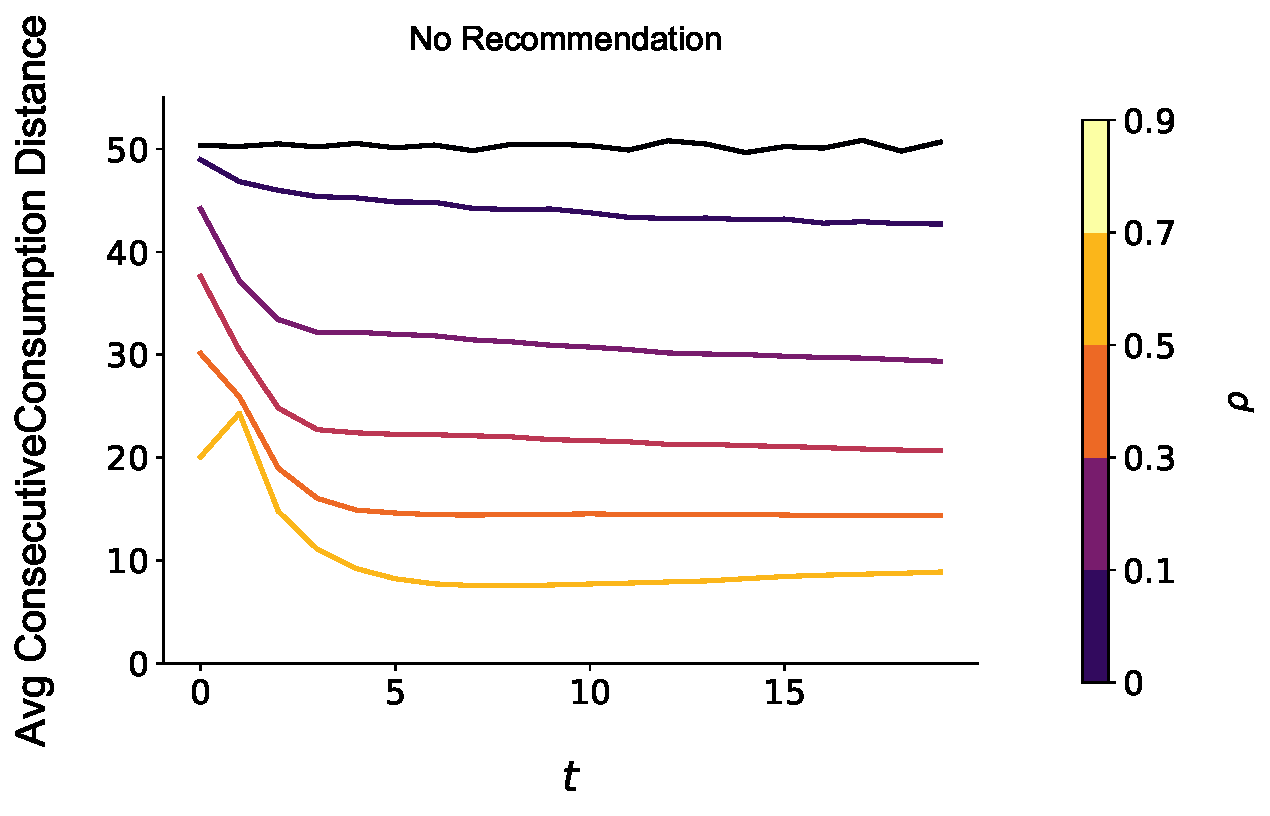
\includegraphics[width=\linewidth]{figures/rho_consumption_dist_N_200T_20.pdf}
\end{subfigure}
\begin{subfigure}{.45\textwidth}
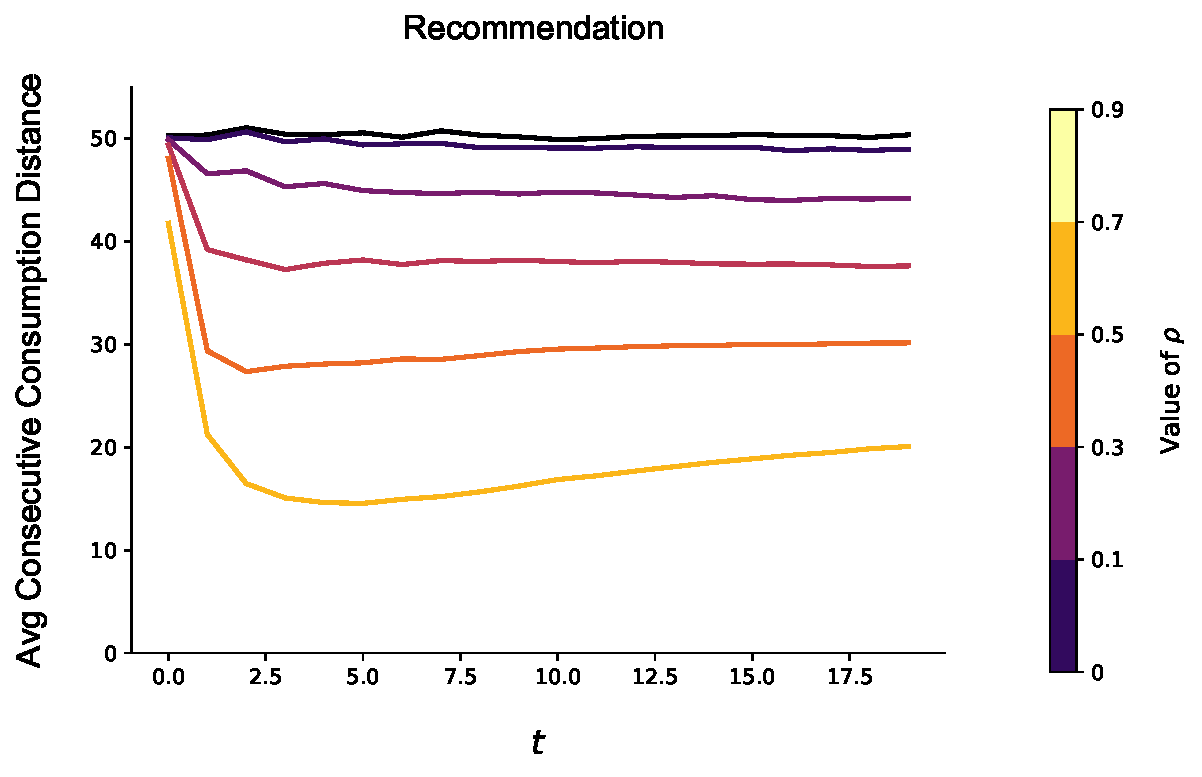
\includegraphics[width=\linewidth]{figures/rho_consumption_dist_N_200T_20_partial.pdf}
\end{subfigure}\\
\begin{subfigure}{.45\textwidth}
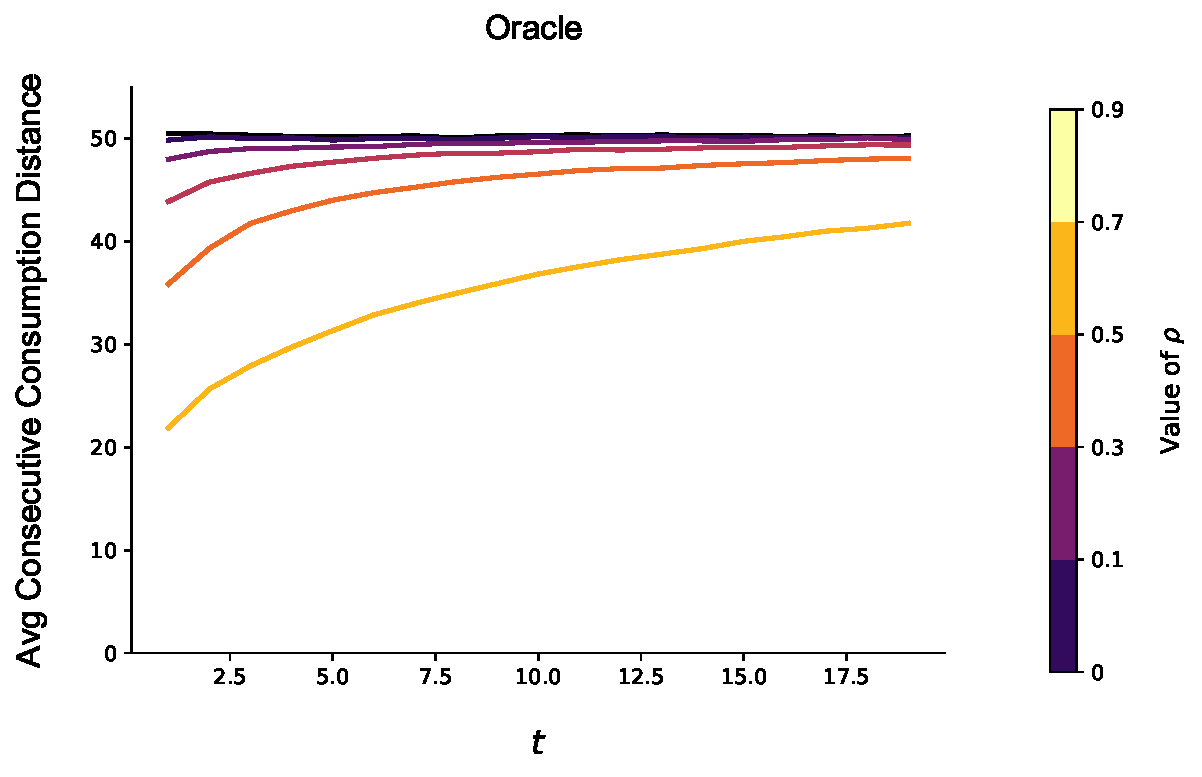
\includegraphics[width=\linewidth]{figures/rho_consumption_dist_N_200T_20_omni.pdf}\\
\end{subfigure}
\caption{Extent of Local Consumption as strength of correlation, $\rho$, varies. \\ No Recommendation (Top Left), Recommendation (Top Right) and Oracle (Bottom)}
\label{fig:local_consumption_across_rho}
\end{figure}

\begin{figure}[H]
\begin{subfigure}{.45\textwidth}
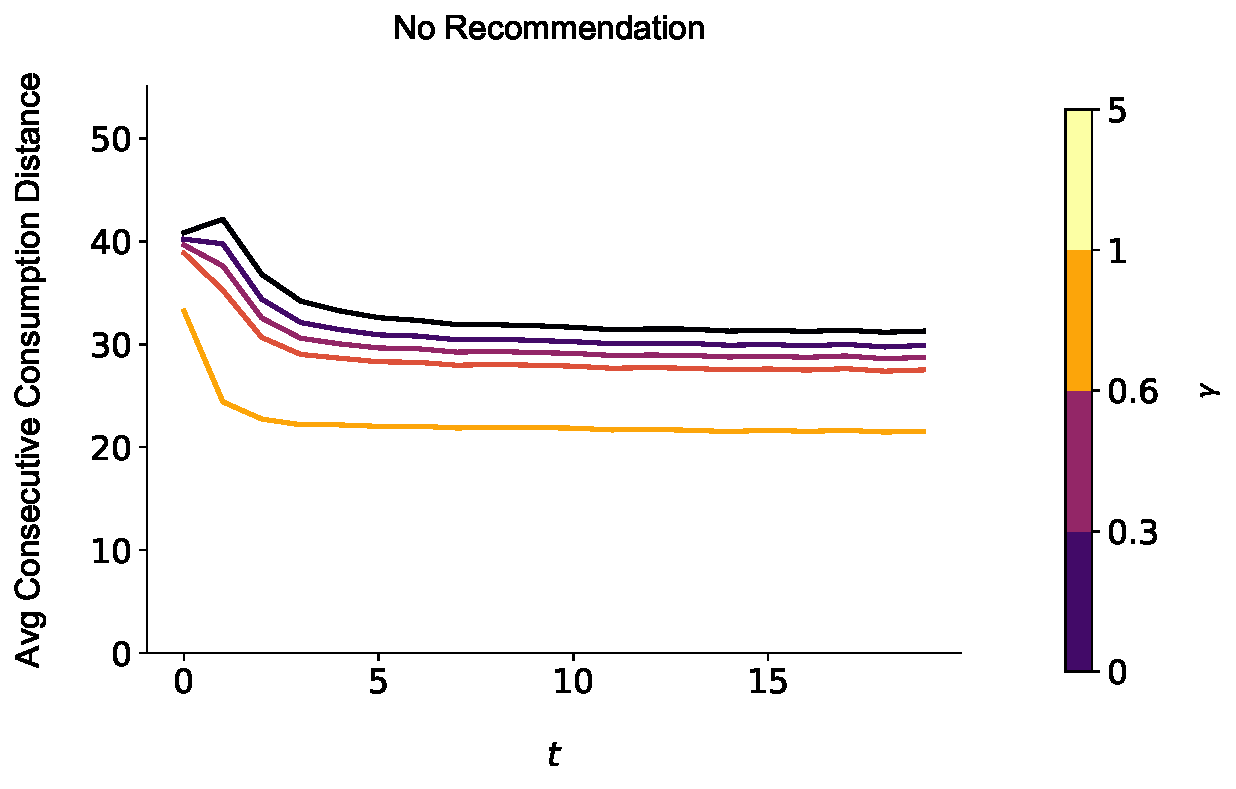
\includegraphics[width=\linewidth]{figures/gamma_consumption_dist_N_200T_20.pdf}
\end{subfigure}
\begin{subfigure}{.45\textwidth}
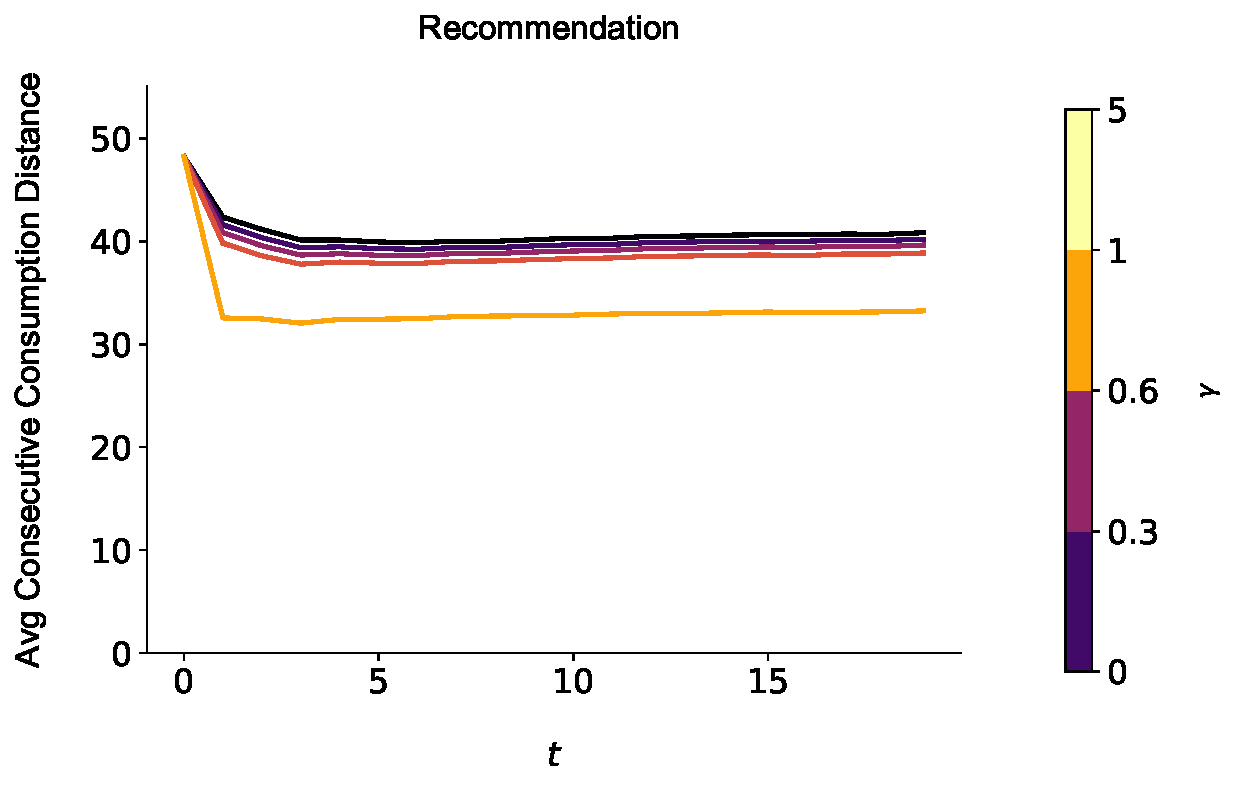
\includegraphics[width=\linewidth]{figures/gamma_consumption_dist_N_200T_20_partial.pdf}
\end{subfigure}\\
\begin{subfigure}{.45\textwidth}
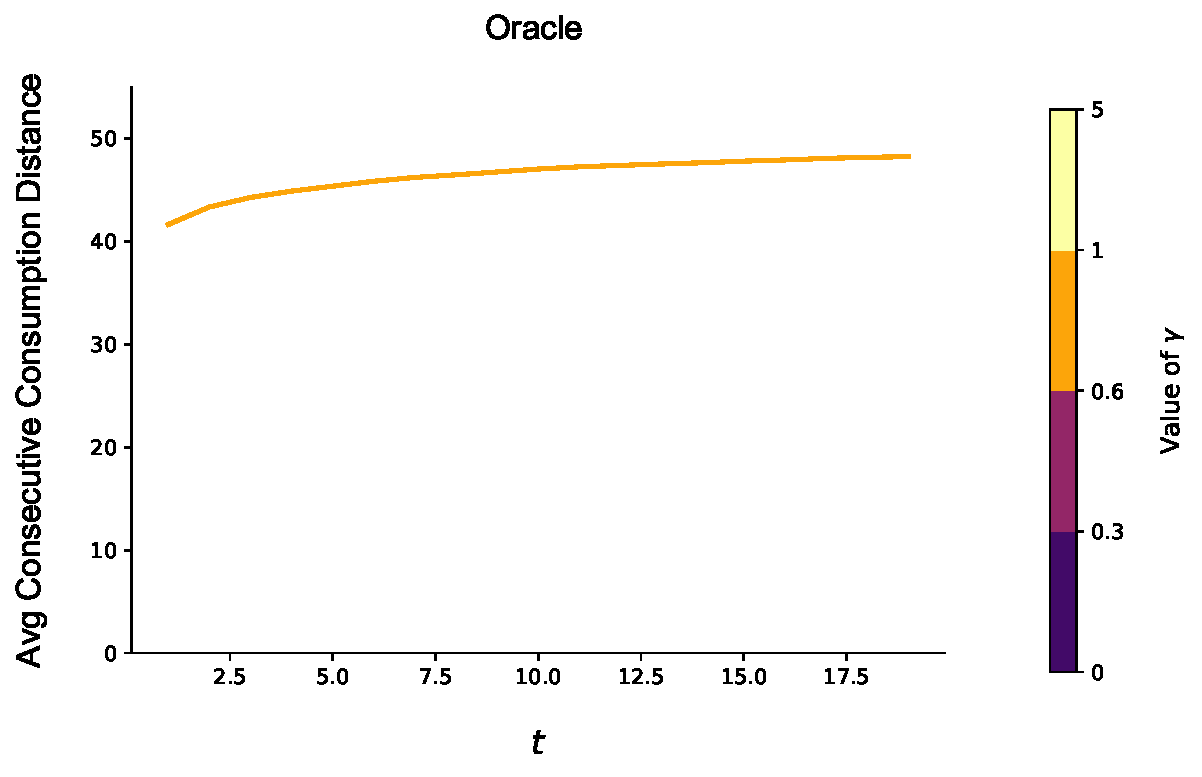
\includegraphics[width=\linewidth]{figures/gamma_consumption_dist_N_200T_20_omni.pdf}\\
\end{subfigure}%
\caption{Effect of Risk Aversion ($\gamma$) on Local Consumption \\ No Recommendation (Top Left), Recommendation (Top Right) and Oracle (Bottom)}
\label{fig:no_rec_risk_aversion}
\end{figure}

\begin{figure}
\begin{subfigure}{.45\linewidth}
  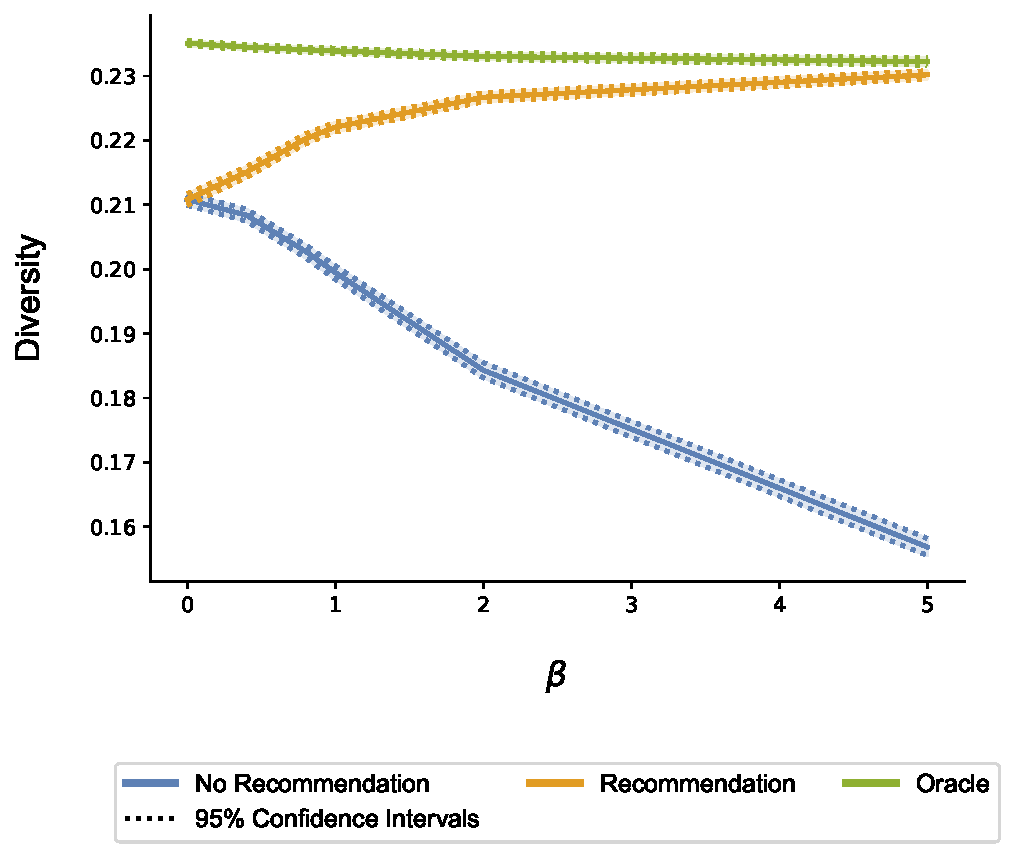
\includegraphics[width=.8\linewidth]{figures/beta_diversity_N_200_T_20.pdf}
\end{subfigure}
\begin{subfigure}{.45\linewidth}
  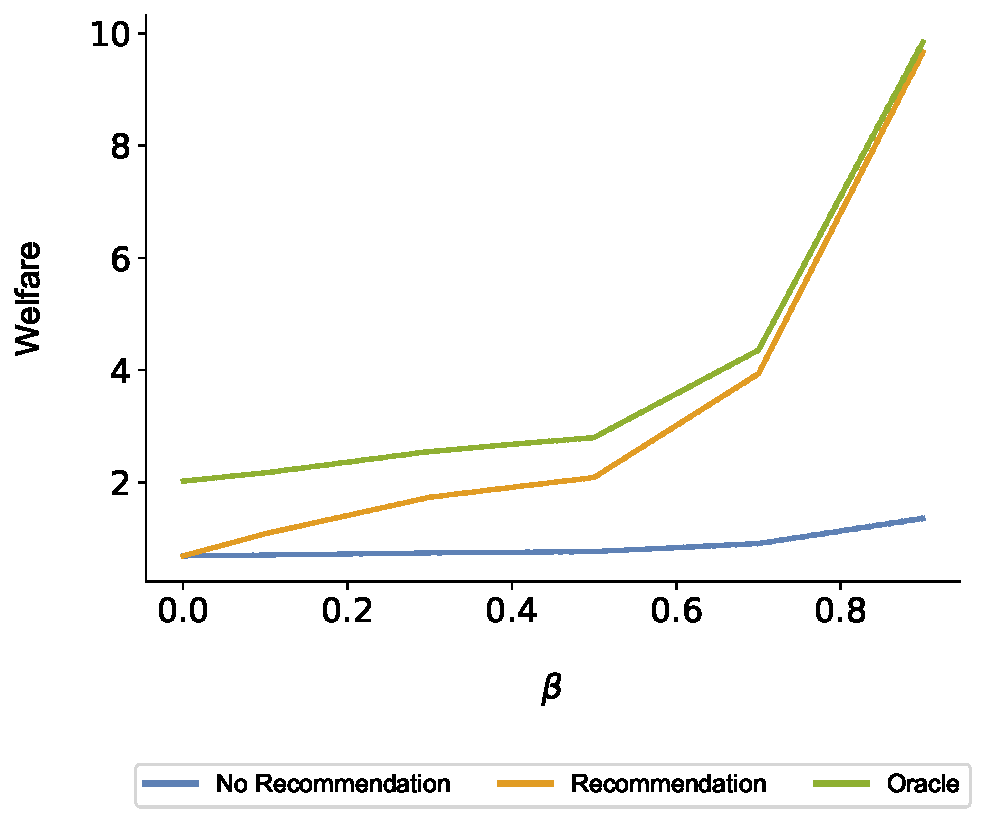
\includegraphics[width=.8\linewidth]{figures/beta_welfare_N_200_T_20.pdf}
\end{subfigure}
\caption{User Welfare and Diversity as the strength of the common value component, $\beta$, varies}\label{fig:diversity_welfare_common_value}
\end{figure}

\begin{figure}[t]
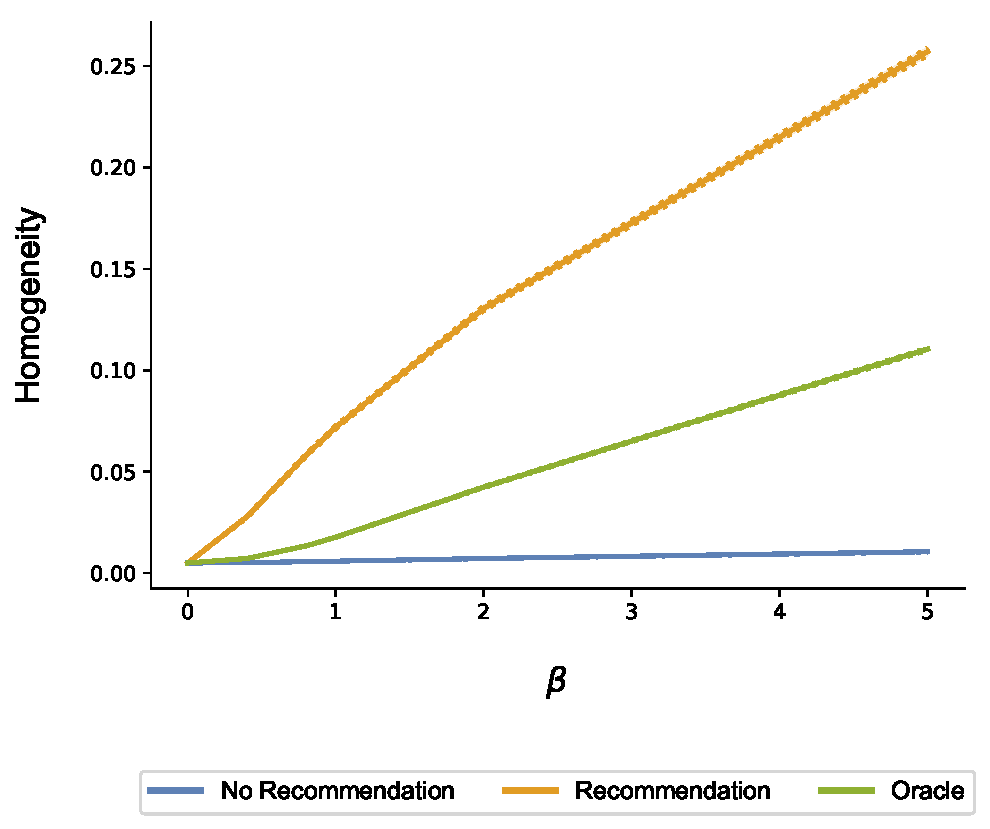
\includegraphics[width=.45\linewidth]{figures/beta_homogeneity_N_200_T_20}
\captionof{figure}{Strength of Recommendation ($\beta$) and Homogeneity}\label{fig:beta_homo}
\end{figure}
\begin{figure}[t]
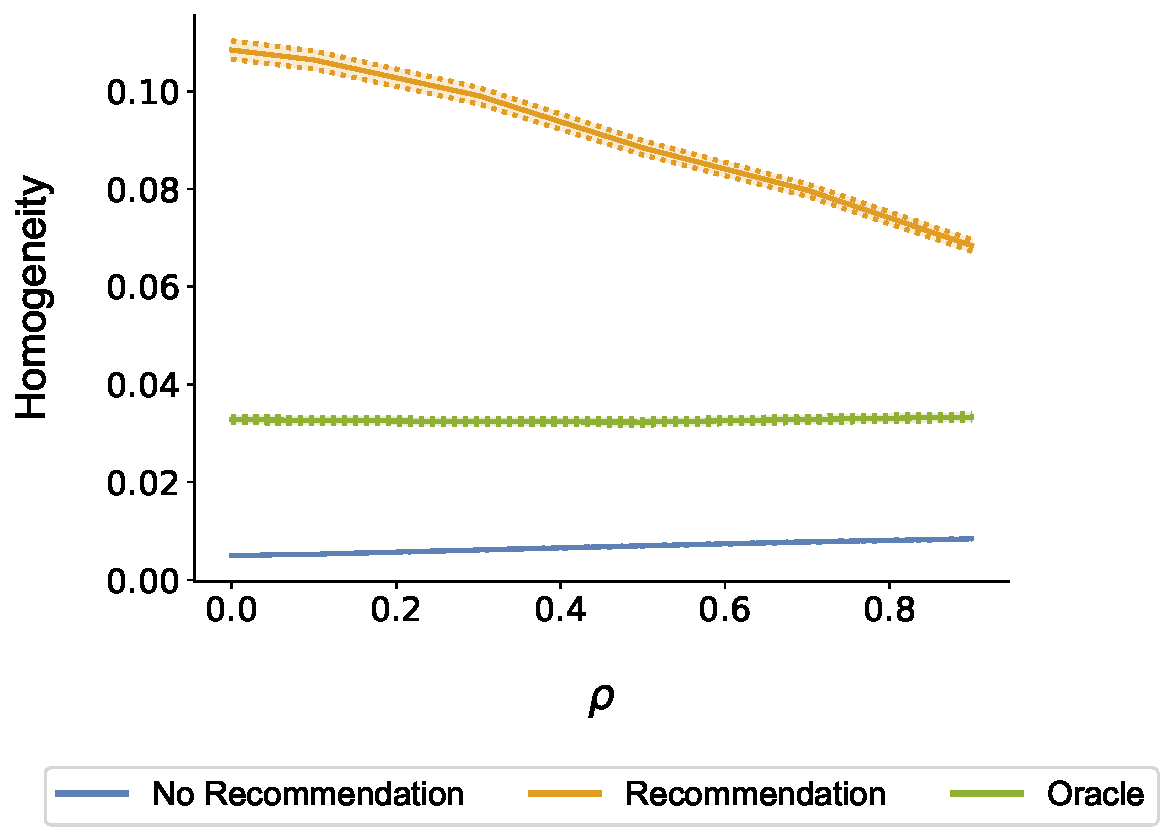
\includegraphics[width=.45\linewidth]{figures/rho_homogeneity_N_200_T_20}
\captionof{figure}{Correlation ($\rho$) and Homogeneity}\label{fig:cor_homo}
\end{figure}

% Bibliography
\bibliographystyle{ACM-Reference-Format}
\bibliography{refs}

\end{document}
